% =============================================================================
% Fig 0 schematic - TikZ source.  Primary version for main.tex.
%
% Two usage modes:
%   (1) Standalone compile -> fig0.pdf, then \includegraphics in main.tex.
%       Just compile this file directly: `pdflatex fig0_schematic.tex`.
%   (2) Inline into main.tex.  Copy the \tikzset block into your preamble
%       (or \input it), then copy the \begin{figure}...\end{figure} block
%       into the body.  See latex_templates.tex for the wrapper.
%
% Two layout variants are provided:
%   Version A (default, active): single-column - figure / \columnwidth.
%   Version B (commented out at the bottom): double-column - figure* /
%   \textwidth, larger font and spacing.  Swap if you want this as the
%   paper's opening figure.
% =============================================================================
\documentclass[tikz,border=2mm]{standalone}
\usepackage{amsmath}
\usepackage[T1]{fontenc}
\usepackage{tikz}
\usetikzlibrary{positioning, arrows.meta, calc, fit, backgrounds, shapes.geometric}

% -----------------------------------------------------------------------------
% Reusable styles (copy this block into main.tex preamble if inlining).
% -----------------------------------------------------------------------------
\tikzset{
    vbox/.style={
        draw=black!70, line width=0.5pt, rounded corners=2pt,
        minimum width=18mm, minimum height=7mm,
        font=\footnotesize, align=center,
        inner sep=2pt, fill=white
    },
    anchor-A0/.style={vbox, fill=black!5},
    anchor-A1/.style={vbox, fill=blue!7},
    anchor-real/.style={vbox, fill=black!3, draw=black!85, line width=0.7pt},
    method-ours/.style={vbox, fill=red!8, draw=red!75!black, line width=0.7pt},
    src/.style={
        font=\scriptsize\itshape, text=black!65,
        align=center, inner sep=1pt
    },
    pipe/.style={
        -{Latex[length=1.4mm, width=1.2mm]},
        line width=0.45pt, draw=black!70
    },
    sumop/.style={
        circle, draw=black!70, line width=0.45pt,
        inner sep=0pt, minimum size=2.6mm,
        font=\scriptsize
    },
    plabel/.style={font=\footnotesize\bfseries, anchor=south west},
    plabelbot/.style={font=\scriptsize, text=black!60, align=center},
    ourbadge/.style={
        font=\scriptsize\bfseries, text=red!75!black,
        fill=red!8, draw=red!75!black, line width=0.4pt,
        rounded corners=1pt, inner sep=1.5pt
    },
}

\begin{document}

% =============================================================================
% Version A: single-column layout (default).
% =============================================================================
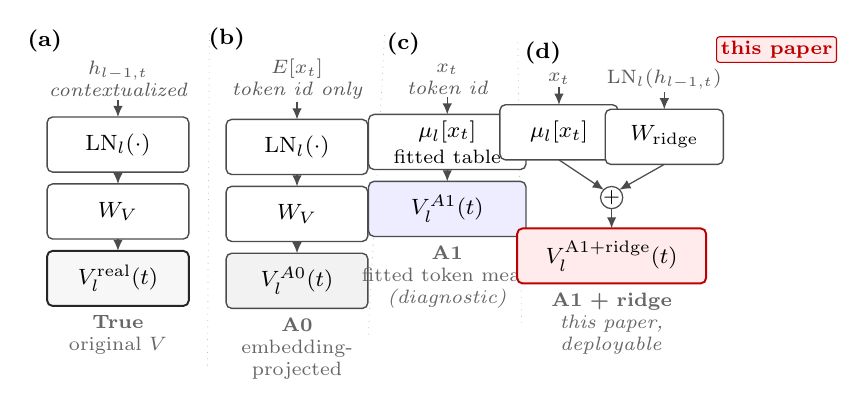
\begin{tikzpicture}[
    panel sep/.style={node distance=2.0mm and 3.5mm},
    inner sep=0pt, outer sep=0pt
]

% ---- Panel (a): true V ----
\node[src] (a-src) {$h_{l-1,t}$\\\textit{contextualized}};
\node[vbox, below=2.2mm of a-src] (a-ln) {$\mathrm{LN}_l(\cdot)$};
\node[vbox, below=1.5mm of a-ln]  (a-wv) {$W_V$};
\node[anchor-real, below=1.5mm of a-wv] (a-v) {$V^{\mathrm{real}}_l(t)$};
\draw[pipe] (a-src) -- (a-ln);
\draw[pipe] (a-ln) -- (a-wv);
\draw[pipe] (a-wv) -- (a-v);
\node[plabel, above left=0.8mm and -2mm of a-src.north west] {(a)};
\node[plabelbot, below=1.2mm of a-v.south, text width=22mm]
    {\textbf{True}\\original $V$};

% ---- Panel (b): A0 ----
\node[src, right=5mm of a-src.east, anchor=west] (b-src) {$E[x_t]$\\\textit{token id only}};
\node[vbox, below=2.2mm of b-src] (b-ln) {$\mathrm{LN}_l(\cdot)$};
\node[vbox, below=1.5mm of b-ln]  (b-wv) {$W_V$};
\node[anchor-A0, below=1.5mm of b-wv] (b-v) {$V_l^{A0}(t)$};
\draw[pipe] (b-src) -- (b-ln);
\draw[pipe] (b-ln) -- (b-wv);
\draw[pipe] (b-wv) -- (b-v);
\node[plabel, above left=0.8mm and -2mm of b-src.north west] {(b)};
\node[plabelbot, below=1.2mm of b-v.south, text width=22mm]
    {\textbf{A0}\\embedding-projected};

% ---- Panel (c): A1 ----
\node[src, right=5mm of b-src.east, anchor=west] (c-src) {$x_t$\\\textit{token id}};
\node[vbox, below=2.2mm of c-src, minimum width=20mm]
    (c-tbl) {$\mu_l[x_t]$\\\scriptsize fitted table};
\node[anchor-A1, below=1.5mm of c-tbl, minimum width=20mm]
    (c-v) {$V_l^{A1}(t)$};
\draw[pipe] (c-src) -- (c-tbl);
\draw[pipe] (c-tbl) -- (c-v);
\node[plabel, above left=0.8mm and -2mm of c-src.north west] {(c)};
\node[plabelbot, below=1.2mm of c-v.south, text width=24mm]
    {\textbf{A1}\\fitted token mean\\\textit{(diagnostic)}};

% ---- Panel (d): A1 + ridge (this paper) ----
\node[src, right=5mm of c-src.east, anchor=west, xshift=2mm]
    (d-src1) {$x_t$};
\node[src, right=4mm of d-src1.east, anchor=west]
    (d-src2) {$\mathrm{LN}_l(h_{l-1,t})$};
\node[vbox, below=2.2mm of d-src1, minimum width=15mm]
    (d-tbl) {$\mu_l[x_t]$};
\node[vbox, below=2.2mm of d-src2, minimum width=15mm]
    (d-ridge) {$W_{\mathrm{ridge}}$};
\node[sumop] (d-sum) at ($(d-tbl)!0.5!(d-ridge) + (0, -8mm)$) {$+$};
\node[method-ours, below=2.5mm of d-sum, minimum width=24mm]
    (d-v) {$V^{\mathrm{A1+ridge}}_l(t)$};
\draw[pipe] (d-src1) -- (d-tbl);
\draw[pipe] (d-src2) -- (d-ridge);
\draw[pipe] (d-tbl.south) -- (d-sum.north west);
\draw[pipe] (d-ridge.south) -- (d-sum.north east);
\draw[pipe] (d-sum) -- (d-v);
\node[plabel, above left=0.8mm and -2mm of d-src1.north west] {(d)};
\node[plabelbot, below=1.2mm of d-v.south, text width=26mm]
    {\textbf{A1 + ridge}\\\textit{this paper, deployable}};
\node[ourbadge, above right=0.5mm and -1mm of d-src2.north east]
    {this paper};

% ---- Panel dividers ----
\begin{scope}[on background layer]
    \draw[dotted, draw=black!25, line width=0.3pt]
        ($(a-src.north east)!0.5!(b-src.north west) + (0, 3mm)$) --
        ($(a-v.south east)!0.5!(b-v.south west)   + (0, -8mm)$);
    \draw[dotted, draw=black!25, line width=0.3pt]
        ($(b-src.north east)!0.5!(c-src.north west) + (0, 3mm)$) --
        ($(b-v.south east)!0.5!(c-v.south west)   + (0, -8mm)$);
    \draw[dotted, draw=black!25, line width=0.3pt]
        ($(c-src.north east)!0.5!(d-src1.north west) + (0, 3mm)$) --
        ($(c-v.south east)!0.5!(d-v.south west)    + (0, -8mm)$);
\end{scope}

\end{tikzpicture}

\end{document}

% =============================================================================
% Version B: double-column (figure*, \textwidth).  To use, replace the
% standalone \begin{document}...\end{document} body above with the picture
% below, OR copy this block into main.tex as a \begin{figure*} ... \end{figure*}.
% =============================================================================
%
% \begin{tikzpicture}[inner sep=0pt, outer sep=0pt]
% \tikzset{
%     vbox/.append style={minimum width=24mm, minimum height=8mm, font=\small},
%     src/.append style={font=\footnotesize\itshape},
%     sumop/.append style={minimum size=3.2mm, font=\small},
%     plabelbot/.append style={font=\footnotesize},
% }
% % (a) true V
% \node[src] (a-src) {$h_{l-1,t}$ \;\textit{(contextualized)}};
% \node[vbox, below=3mm of a-src] (a-ln) {$\mathrm{LN}_l(\cdot)$};
% \node[vbox, below=2mm of a-ln]  (a-wv) {$W_V$};
% \node[anchor-real, below=2mm of a-wv] (a-v) {$V^{\mathrm{real}}_l(t)$};
% \draw[pipe] (a-src) -- (a-ln);
% \draw[pipe] (a-ln) -- (a-wv);
% \draw[pipe] (a-wv) -- (a-v);
% \node[plabel, above left=1mm and -3mm of a-src.north west] {(a)};
% \node[plabelbot, below=2mm of a-v.south, text width=30mm]
%     {\textbf{True $V$}\\original construction};
% % (b) A0
% \node[src, right=10mm of a-src.east, anchor=west] (b-src) {$E[x_t]$ \;\textit{(token only)}};
% \node[vbox, below=3mm of b-src] (b-ln) {$\mathrm{LN}_l(\cdot)$};
% \node[vbox, below=2mm of b-ln]  (b-wv) {$W_V$};
% \node[anchor-A0, below=2mm of b-wv] (b-v) {$V_l^{A0}(t)$};
% \draw[pipe] (b-src) -- (b-ln);
% \draw[pipe] (b-ln) -- (b-wv);
% \draw[pipe] (b-wv) -- (b-v);
% \node[plabel, above left=1mm and -3mm of b-src.north west] {(b)};
% \node[plabelbot, below=2mm of b-v.south, text width=30mm]
%     {\textbf{Anchor $A0$}\\embedding-projected\\token table};
% % (c) A1
% \node[src, right=10mm of b-src.east, anchor=west] (c-src) {$x_t$ \;\textit{(token id)}};
% \node[vbox, below=3mm of c-src, minimum width=28mm]
%     (c-tbl) {$\mu_l[x_t]$ \,\;\scriptsize (fitted)};
% \node[anchor-A1, below=2mm of c-tbl, minimum width=28mm]
%     (c-v) {$V_l^{A1}(t)$};
% \draw[pipe] (c-src) -- (c-tbl);
% \draw[pipe] (c-tbl) -- (c-v);
% \node[plabel, above left=1mm and -3mm of c-src.north west] {(c)};
% \node[plabelbot, below=2mm of c-v.south, text width=32mm]
%     {\textbf{Anchor $A1$}\\fitted per-token mean\\\textit{(diagnostic only)}};
% % (d) A1 + ridge
% \node[src, right=10mm of c-src.east, anchor=west, xshift=3mm]
%     (d-src1) {$x_t$};
% \node[src, right=8mm of d-src1.east, anchor=west]
%     (d-src2) {$\mathrm{LN}_l(h_{l-1,t})$};
% \node[vbox, below=3mm of d-src1, minimum width=20mm]
%     (d-tbl) {$\mu_l[x_t]$};
% \node[vbox, below=3mm of d-src2, minimum width=20mm]
%     (d-ridge) {$W_{\mathrm{ridge}}$};
% \node[sumop] (d-sum) at ($(d-tbl)!0.5!(d-ridge) + (0, -10mm)$) {$+$};
% \node[method-ours, below=3mm of d-sum, minimum width=32mm]
%     (d-v) {$V^{\mathrm{A1+ridge}}_l(t)$};
% \draw[pipe] (d-src1) -- (d-tbl);
% \draw[pipe] (d-src2) -- (d-ridge);
% \draw[pipe] (d-tbl.south) -- (d-sum.north west);
% \draw[pipe] (d-ridge.south) -- (d-sum.north east);
% \draw[pipe] (d-sum) -- (d-v);
% \node[plabel, above left=1mm and -3mm of d-src1.north west] {(d)};
% \node[plabelbot, below=2mm of d-v.south, text width=36mm]
%     {\textbf{$A1 +$ ridge correction}\\\textit{deployable form (\S\ref{sec:results})}};
% \node[ourbadge, above right=1mm and -1mm of d-src2.north east] {this paper};
% % dividers
% \begin{scope}[on background layer]
%     \foreach \left/\right in {a/b, b/c, c/d}{
%         \draw[dotted, draw=black!25, line width=0.3pt]
%             ($(\left-src.north east)!0.5!(\right-src.north west) + (0, 4mm)$) --
%             ($(\left-v.south east)!0.5!(\right-v.south west) + (0, -10mm)$);
%     }
% \end{scope}
% \end{tikzpicture}
